\documentclass[14pt, a4paper]{extarticle}
\usepackage{GOST}
\usepackage{array}
\usepackage{verbatim}
\usepackage[detect-all]{siunitx}
\usepackage{amsmath}
\usepackage{amssymb}
\usepackage[utf8]{inputenc}
\usepackage{hyperref}

\usepackage{ifthen}


\usepackage{tempora}



\makeatletter
\renewcommand\@biblabel[1]{#1.}
\makeatother

% Для листинга кода:
\usepackage{listings}
\lstset{ %
	language=c,                 % выбор языка для подсветки (здесь это С)
	basicstyle=\small\sffamily, % размер и начертание шрифта для подсветки кода
	numbers=left,               % где поставить нумерацию строк (слева\справа)
	numberstyle=\tiny,           % размер шрифта для номеров строк
	stepnumber=1,                   % размер шага между двумя номерами строк
	numbersep=5pt,                % как далеко отстоят номера строк от подсвечиваемого кода
	showspaces=false,            % показывать или нет пробелы специальными отступами
	showstringspaces=false,      % показывать или нет пробелы в строках
	showtabs=false,             % показывать или нет табуляцию в строках
	frame=single,              % рисовать рамку вокруг кода
	tabsize=2,                 % размер табуляции по умолчанию равен 2 пробелам
	captionpos=t,              % позиция заголовка вверху [t] или внизу [b] 
	breaklines=true,           % автоматически переносить строки (да\нет)
	breakatwhitespace=false, % переносить строки только если есть пробел
	escapeinside={\#*}{*)}   % если нужно добавить комментарии в коде
}


%для графиков
\usepackage{pgfplots}
\usepackage{filecontents}
\usetikzlibrary{datavisualization}
\usetikzlibrary{datavisualization.formats.functions}

\begin{document}
	
	\begin{table}[ht]
		\centering
		\begin{tabular}{|c|p{400pt}|} 
			\hline
			\begin{tabular}[c]{@{}c@{}} 
\includegraphics[scale=1]{source/baum.jpg} \\\end{tabular} &
			\footnotesize\begin{tabular}[c]{@{}c@{}}\textbf{Министерство~науки~и~высшего~образования~Российской~Федерации}\\\textbf{Федеральное~государственное~бюджетное~образовательное~учреждение}\\\textbf{~высшего~образования}\\\textbf{«Московский~государственный~технический~университет}\\\textbf{имени~Н.Э.~Баумана}\\\textbf{(национальный~исследовательский~университет)»}\\\textbf{(МГТУ~им.~Н.Э.~Баумана)}\\\end{tabular}  \\
			\hline
		\end{tabular}
	\end{table}
	\noindent\rule{\textwidth}{4pt}
	\noindent\rule[14pt]{\textwidth}{1pt}
	\hfill 
	\noindent
	\makebox{ФАКУЛЬТЕТ~}%
	\makebox[\textwidth][l]{\underline{~«Информатика и системы управления»~~~~~~~~~~~~~~~~~~~~~~~~~~~~~~~~~}}%
	\\
	\noindent
	\makebox{КАФЕДРА~}%
	\makebox[\textwidth][l]{\underline{~«Программное обеспечение ЭВМ и информационные технологии»~}}%
	\\
	
	\begin{center}
		\vspace{1.5cm}
		{\bf\huge Отчёт\par}
		{\bf\Large по лабораторной работе № 2\par}
		\vspace{0.7cm}
	\end{center}
	
	
	\noindent
	\makebox{\large{\bf Название:}~~~}
	\makebox[\textwidth][l]{\large\underline{~~~~~~Защищенный режим~~~~~}}\\
	
	\noindent
	\makebox{\large{\bf Дисциплина:}~~~}
	\makebox[\textwidth][l]{\large\underline{~Операционные системы~}}\\
	
	\vspace{1.5cm}
	\noindent
	\begin{tabular}{l c c c c c}
		Студент      & ~ИУ7-55Б~               & \hspace{2.5cm} & \hspace{2cm}                 & &  Д.В. 
		Сусликов \\\cline{2-2}\cline{4-4} \cline{6-6} 
		\hspace{3cm} & {\footnotesize(Группа)} &                & {\footnotesize(Подпись, дата)} & & {\footnotesize(И.О. Фамилия)}
	\end{tabular}
	
	\noindent
	\begin{tabular}{l c c c c}
		Преподаватель & \hspace{5cm}   & \hspace{2cm}                 & & ~~~~~~Н.Ю. Рязанова~~~~~~\\\cline{3-3} \cline{5-5} 
		\hspace{3cm}  &                & {\footnotesize(Подпись, дата)} & & {\footnotesize(И.О. Фамилия)}
	\end{tabular}
	
	\vspace{0.6cm}
	\begin{center}	
		\vfill
		\large \textit {Москва, 2020}
	\end{center}
	
	\thispagestyle {empty}
	\pagebreak
	
	% СОДЕРЖАНИЕ 
	\clearpage
	\tableofcontents
	
	
	% ВВЕДЕНИЕ
	\clearpage
	\section{Листинг программы}
	Ниже показан Листинг программы.
	\begin{lstlisting}	
		.586p
		
		seg_descr struc     
		lim 	dw 0	
		base_l 	dw 0	
		base_m 	db 0	
		attr_1	db 0	
		attr_2	db 0	
		base_h 	db 0	
		seg_descr ends
		
		
		int_descr struc 
		offs_l 	dw 0  
		sel		dw 0  
		cntr    db 0  
		attr	db 0  
		offs_h 	dw 0 
		int_descr ends
		
		
		seg_stack segment  para stack 'STACK'
		stack_start	db	256 dup(?)
		stack_size = $-stack_start
		seg_stack 	ENDS
		
		seg_data segment para 'DATA'
		gdt_null  seg_descr <>
		
		gdt_flatDS	seg_descr <0FFFFh, 0, 0, 10010010b, 10001111b, 0>
		
		gdt_16bitCS	seg_descr <seg_rm_size-1, 0, 0, 10011000b, 00000000b, 0> 
		
		gdt_32bitCS	seg_descr <seg_pm_size-1, 0, 0, 10011000b, 01000000b, 0>
		
		gdt_32bitDS	seg_descr <data_size-1, 0, 0, 10010010b, 01000000b, 0>
		
		gdt_32bitSS	seg_descr <stack_size-1, 0, 0, 10010110b, 01000000b, 0>
		
		gdt_PM_videobuffer_32bit seg_descr <4095, 8000h, 0Bh, 10010010b, 01000000b, 0>
		
		gdt_size = $-gdt_null 
		
		gdtr	df 0	
		
		sel_flatDS      equ    8   
		sel_16bitCS     equ   16   
		sel_32bitCS     equ   24
		sel_32bitDS     equ   32
		sel_32bitSS     equ   40
		sel_VideoBuf    equ   48
		
		IDT	label byte
		
		int_descr 13 dup (<0, sel_32bitCS, 0, 10001111b, 0>) 
		trap_13 int_descr <0, sel_32bitCS, 0, 10001111b, 0>  
		int_descr 18 dup (<0, sel_32bitCS, 0, 10001111b, 0>) 
		
		int08 int_descr <0, sel_32bitCS, 0, 10001110b, 0> 
		
		int09 int_descr	<0, sel_32bitCS, 0, 10001110b, 0> 
		
		idt_size = $-IDT 
		
		idtr	df 0 
		
		idtr_real dw	3FFh, 0, 0 
		
		master	db 0					 
		slave	db 0					 
		
		mark_08	dw 0				 
		time_08	dd 0				
		screen_pos 	dd 2 * 80       
		
		ascii	db 0, 27 
		db '1234567890-+', 8 
		db 9, 'QWERTYUIOP[]', 0 
		db 0,  'ASDFGHJKL', 59, 39, 96, 0
		db     '\ZXCVBNM,./', 0
		db 0, 0, 0, 0, ' ', 0, 0
		
		msg_rm   db 'Real Mode', 10, '$'
		msg_pm db 'Protected Mode', 10, '$'
		msg_skip db 10,10,10, '$'
		
		data_size = $-gdt_null
		seg_data ends
		
		seg_pm segment para public 'CODE' use32
		assume cs:seg_pm, ds:seg_data, ss:seg_stack
		pm_start:
		mov	ax, sel_32bitDS 
		mov	ds, ax
		mov	ax, sel_VideoBuf
		mov	es, ax
		mov	ax, sel_32bitSS
		mov	ss, ax
		mov	eax, stack_size
		mov	esp, eax
		
		sti 
		call calc_memory_amount
		
		start_08:
		test mark_08, 1
		jz start_08
		
		
		cli 
		
		db	0EAh
		dd	offset real_mode_return
		dw	sel_16bitCS
		
		new_int08 proc uses eax 
		mov  eax, time_08
		
		call timing
		
		inc eax
		mov time_08, eax
		
		mov	al, 20h 
		out	20h, al
		
		iretd
		new_int08 endp
		
		new_int09 proc uses eax ebx edx 
		in	al, 60h      
		
		cmp	al, 1Ch 	 
		jne	print_key  
		or mark_08, 1   
		jmp leave_stop
		
		print_key:
		cmp al, 80h  
		ja leave_stop 	
		
		xor ah, ah	    
		xor ebx, ebx
		mov bx, ax
		
		mov dl, ascii[ebx]   
		mov ebx, screen_pos   
		mov es:[ebx], dl
		
		add ebx, 2          
		mov screen_pos, ebx
		
		leave_stop: 
		in	al, 61h 
		or	al, 80h 
		out	61h, al 
		and al, 7Fh 
		out	61h, al
		
		mov	al, 20h 
		out	20h, al
		
		iretd
		new_int09 endp
		
		plug_trap13:
		pop eax
		iretd
		
		
		to_ascii proc
		cmp dl, 10
		jl number
		add dl, 'A' - '0' - 10 
		number:
		add dl, '0' 
		ret
		to_ascii endp
		
		print_by_eax proc uses ecx ebx edx     
		add ebx, 10h 
		mov ecx, 8   
		print_eax:  
		mov dl, al
		and dl, 0Fh       
		call to_ascii     
		mov es:[ebx], dl 
		ror eax, 4        
		sub ebx, 2       
		loop print_eax
		ret
		print_by_eax endp
		
		calc_memory_amount proc uses ds eax ebx
		mov ax, sel_flatDS
		mov ds, ax
		mov ebx, 100001h 
		mov dl, 12 
		mov	ecx, 0FFEFFFFEh
		
		amount:
		mov dh, ds:[ebx] 
		mov ds:[ebx], dl 
		cmp ds:[ebx], dl 
		jnz mem_end
		
		mov	ds:[ebx], dh 
		inc ebx
		loop amount
		
		mem_end:
		mov eax, ebx
		xor edx, edx
		
		mov ebx, 100000h 
		div ebx
		
		mov ebx, 0
		call print_by_eax
		
		mov ebx, 20
		mov al, 'M'
		mov es:[ebx], al
		
		mov ebx, 22
		mov al, 'B'
		mov es:[ebx], al
		ret
		calc_memory_amount endp
		
		print_time proc uses eax ebx ecx edx
		mov al, dl
		xor ecx, ecx
		
		add ebx, 4
		mov cx, 2
		
		mov dl, 10
		print_numeral:
		xor ah, ah
		div dl
		add ah, '0'
		mov es:[ebx], ah 
		sub ebx, 2
		loop print_numeral
		ret
		print_time endp
		
		timing proc uses eax ebx ecx edx 
		mov ecx, 65536
		xor edx, edx
		mul ecx
		mov ecx, 1193180
		div ecx
		
		xor edx, edx
		mov ecx, 60
		div ecx
		
		mov ebx, 80
		call print_time
		
		mov dh, ':'
		mov es:[ebx], dh
		sub ebx, 6
		
		xor edx, edx
		div ecx
		call print_time
		
		mov dh, ':'
		mov es:[ebx], dh
		sub ebx, 6
		xor dh, dh
		
		mov dl, al
		call print_time
		
		ret
		timing endp
		
		seg_pm_size = $-pm_start 	
		seg_pm ends
		
		seg_rm segment para public 'CODE' use16
		assume cs:seg_rm, ds:seg_data, ss: seg_stack
		
		start:
		mov ax, seg_data
		mov ds, ax
		
		mov ax, seg_pm
		mov es, ax
		
		mov ah, 09h
		lea dx, msg_rm
		int 21h  
		
		mov ah, 09h
		lea dx, msg_pm
		int 21h
		
		push eax
		mov ah, 10h
		int 16h
		pop eax
		
		xor	eax, eax
		mov	ax, seg_rm 
		shl eax, 4                       
		mov word ptr gdt_16bitCS.base_l, ax  
		shr eax, 16                       
		mov byte ptr gdt_16bitCS.base_m, al  
		mov byte ptr gdt_16bitCS.base_h, ah  
		
		
		mov ax, seg_pm
		shl eax, 4                        
		mov word ptr gdt_32bitCS.base_l, ax  
		shr eax, 16                       
		mov byte ptr gdt_32bitCS.base_m, al  
		mov byte ptr gdt_32bitCS.base_h, ah  
		
		
		mov ax, seg_data
		shl eax, 4                       
		mov word ptr gdt_32bitDS.base_l, ax  
		shr eax, 16                       
		mov byte ptr gdt_32bitDS.base_m, al  
		mov byte ptr gdt_32bitDS.base_h, ah  
		
		
		mov ax, seg_stack
		shl eax, 4                        
		mov word ptr gdt_32bitSS.base_l, ax  
		shr eax, 16                       
		mov byte ptr gdt_32bitSS.base_m, al  
		mov byte ptr gdt_32bitSS.base_h, ah 
		
		
		mov ax, seg_data
		shl eax, 4
		add	eax, offset gdt_null 
		
		mov	dword ptr gdtr + 2, eax	    
		mov word ptr  gdtr, gdt_size-1	
		lgdt fword ptr gdtr 
		
		
		lea eax, es:plug_trap13
		mov	trap_13.offs_l, ax 
		shr	eax, 16             
		mov	trap_13.offs_h, ax
		
		lea eax, es:new_int08
		mov	int08.offs_l, ax 
		shr	eax, 16
		mov	int08.offs_h, ax 
		
		lea eax, es:new_int09
		mov	int09.offs_l, ax 
		shr	eax, 16            
		mov	int09.offs_h, ax 
		
		mov ax, seg_data
		shl eax, 4
		add	eax, offset IDT
		
		
		mov	 dword ptr idtr + 2, eax	
		mov  word ptr  idtr, idt_size-1
		
		in	al, 21h	
		mov	master, al
		in	al, 0A1h
		mov	slave, al
		mov	al, 11h
		out	20h, al
		
		mov	al, 32
		out	21h, al
		mov	al, 4						
		out	21h, al
		mov	al, 1
		out	21h, al
		
		mov	al, 0FCh
		out	21h, al
		
		mov	al, 0FFh
		out	0A1h, al
		
		cli         
		in	al, 70h 
		or	al, 80h
		out	70h, al
		
		lidt fword ptr idtr
		
		in	al, 92h						
		or	al, 2						
		out	92h, al						
		
		push ds
		mov	ax, 40h
		mov	ds, ax
		mov eax, dword ptr ds:[6Ch] 
		pop ds
		mov dword ptr time_08, eax
		
		
		mov	eax, cr0
		or eax, 1    
		mov	cr0, eax
		
		db	66h
		db	0EAh
		dd	offset pm_start
		dw	sel_32bitCS
		
		real_mode_return:
		mov	eax, cr0
		and	al, 0FEh
		mov	cr0, eax
		
		db	0EAh
		dw	$+4
		dw	seg_rm
		
		mov	eax, seg_data	
		mov	ds, ax          
		mov eax, seg_pm
		mov	es, ax
		mov	ax, seg_stack
		mov	ss, ax
		mov	ax, stack_size
		mov	sp, ax
		
		mov	al, 11h						
		out	20h, al						
		mov	al, 8    				    
		out	21h, al						
		mov	al, 4						
		out	21h, al                    
		mov	al, 1						
		out	21h, al                     
		
		mov	al, master 
		out	21h, al
		mov	al, slave
		out	0A1h, al
		
		lidt	fword ptr idtr_real
		
		in	al, 70h 
		and	al, 7FH
		out	70h, al
		sti     
		
		mov ah, 09h
		lea dx, msg_rm
		int 21h
		
		mov	ax, 4C00h
		int	21h
		
		seg_rm_size = $-start 	
		seg_rm	ends
		end start
	\end{lstlisting}
	\newpage
	
	\section{Пример работы}
	\begin{figure}[h!]
		\centering{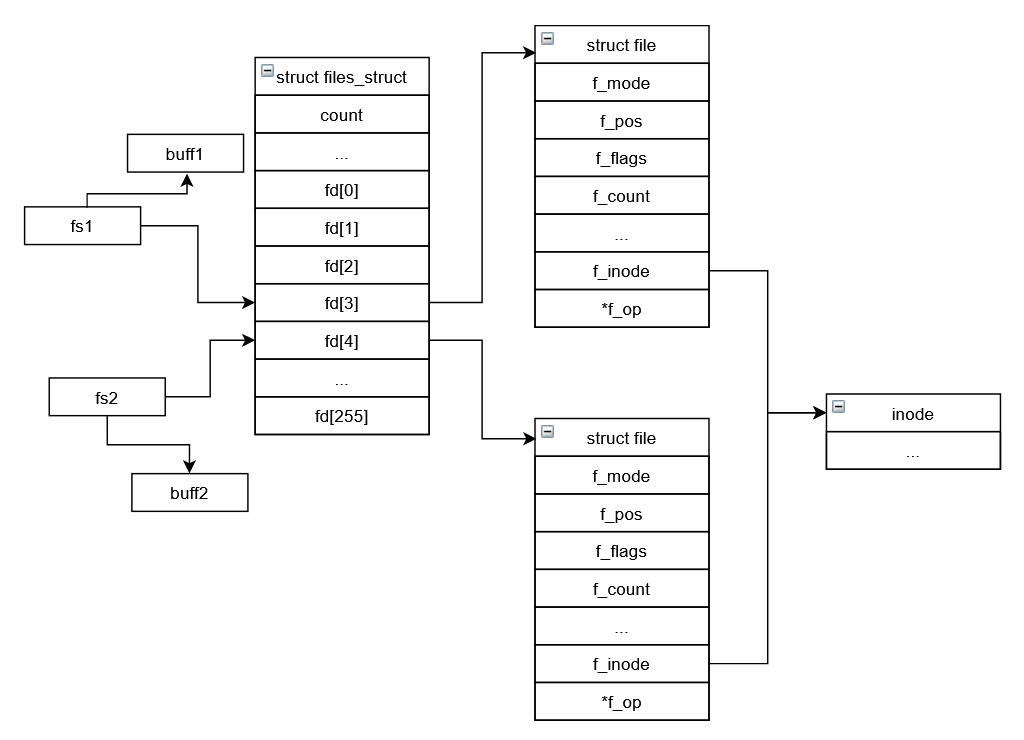
\includegraphics[scale=0.7]{source/1.jpg}}
		\caption{Пример работы}
	\end{figure}
	
	\begin{figure}[h!]
		\centering{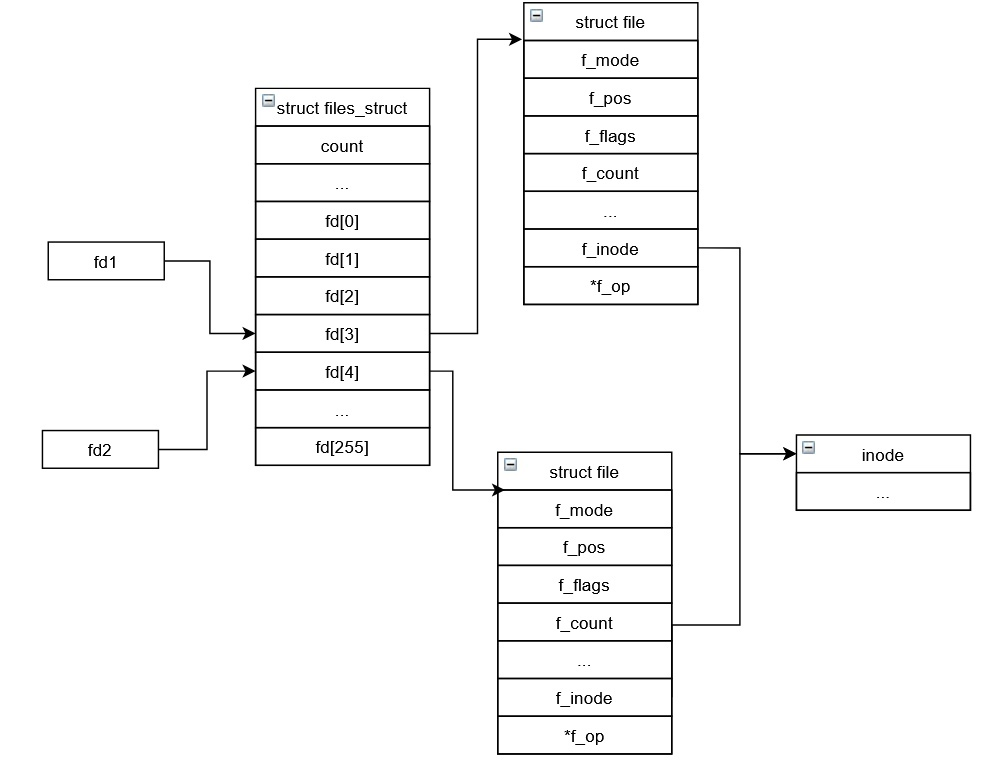
\includegraphics[scale=0.7]{source/2.jpg}}
		\caption{Пример работы}
	\end{figure}

	\begin{figure}[h!]
		\centering{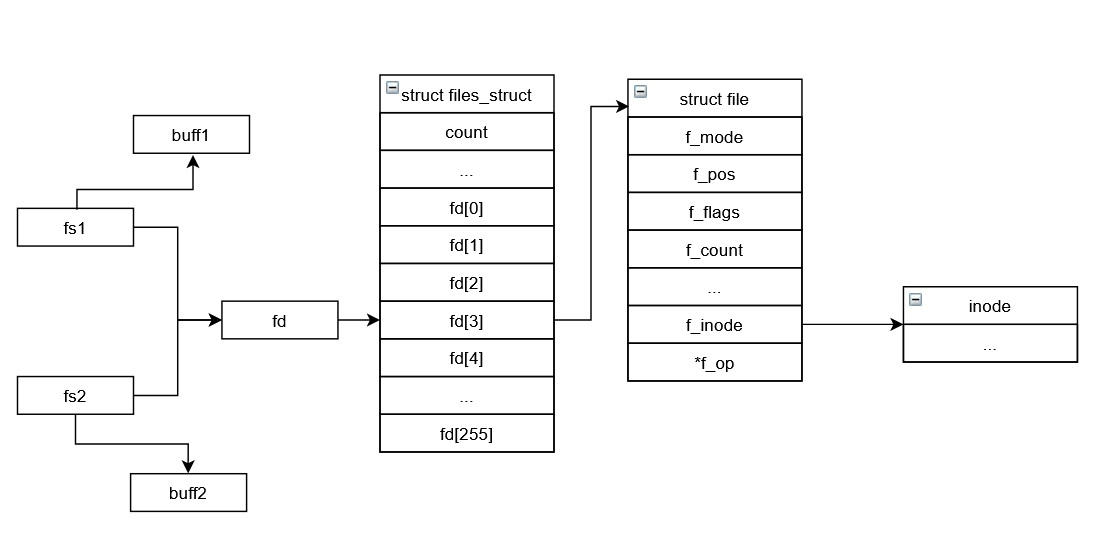
\includegraphics[scale=0.7]{source/3.jpg}}
		\caption{Пример работы}
	\end{figure}

	\begin{figure}[h!]
		\centering{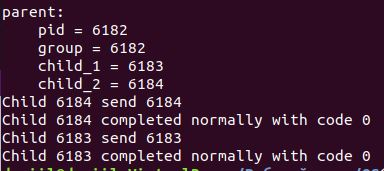
\includegraphics[scale=0.7]{source/4.jpg}}
		\caption{Пример работы}
	\end{figure}

\end{document}